\documentclass[12pt,a4paper]{article}
\usepackage{fullpage}
\pagestyle{plain}
% choose any of the following packages to support AmsTeX
%\usepackage{amsmath,amssymb,amsfonts,mathrsfs,mathptm,bm,mathtools}
% choose the following package to insert eps figures
% for png, jpg or pdf figures, use pdflatex
\usepackage{float}
\usepackage{graphicx}
\graphicspath{{./img}}

\newcommand{\question}[1]{\bigskip\noindent{\textbf{Q{#1} solution}}}

% set HW number
\newcommand{\HWnum}{3}
% specify first and last name and the ID number of students in the group
% append asterix to indicate who is making the submission
\newcommand{\StudentA}{Hanggang Zhu$^\ast$, 3200110457}
\newcommand{\StudentB}{Suhao Wang, 3200110777}
\newcommand{\StudentC}{Lumeng Xu 3200110184}

% ===============================================================
\begin{document}

%%% header
{\noindent \rule{\linewidth}{0.2mm}}
\noindent{ECE 374, ZJUI, Spring 2023\hfill%
  \textbf{\large H{}W\HWnum\ Solutions} \hfill \today\smallskip}

\noindent{\hfill \StudentA, \StudentB, and \StudentC \hfill}
\\[-0.2cm]{\noindent \rule{\linewidth}{0.2mm}}
%%% end header


\question{7.A}

The follwing NFA accpets the language. On reading 3,7,4 at states $q_0,q_1,q_2$ respectively, The NFA can go to next state. In all states the NFA can stay at current state reading any character. But accepting state is reached only if $3,7,4$ are read as a subsequence.


\begin{figure}[hbt!]
	\centering
	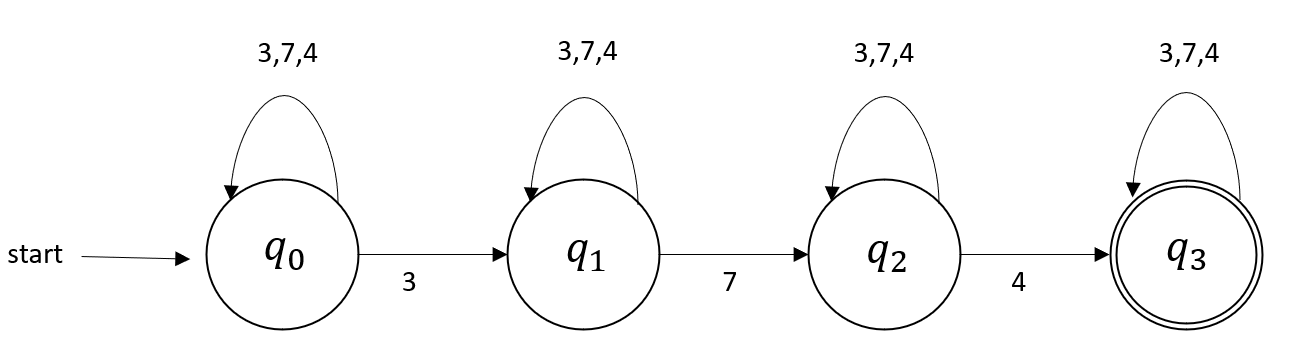
\includegraphics[width = 0.65\textwidth]{Q-7A}
\end{figure}

\question{7.B}

The follwing NFA accepts the language. The state is represented as $w_1,w_2$, which means string \textbf{ends with} $w_1,w_2$ if $\vline\ w\ \vline \neq 3$  and \textbf{contains} $w$ if $\vline\ w\ \vline = 3$. $w_1$ stands for substring $374$ and $w_2$ stands for substring $473$. If no matched string is found at the end of string, it's represented by $\epsilon$. The basic logic is to track the end string and once a substring is observed, mark it as observed and keep tracking the other substring. Accpeting state is reached if and only if both $374$ and $473$ are contained.

\begin{figure}[hbt!]
	\centering
	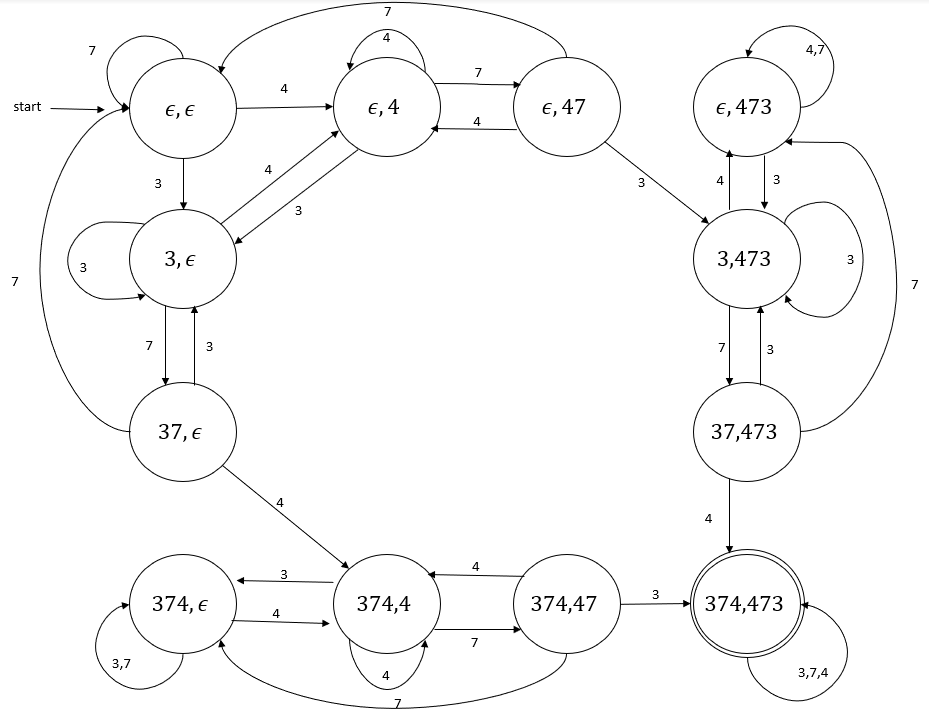
\includegraphics[width = 0.8\textwidth]{Q-7B}
\end{figure}

\question{7.C}

The follwing NFA accepts the language. The state is represents what the string ends with. All strings are accepted but if $4$ is read at state $37$, then there will be a $374$ substring and this won't be accpeted by the NFA.

\begin{figure}[hbt!]
	\centering
	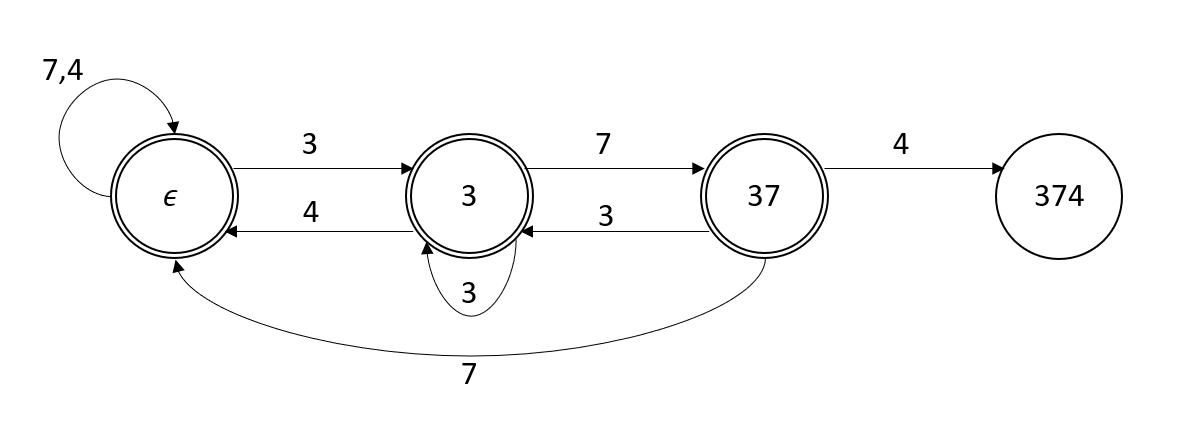
\includegraphics[width = 1\textwidth]{Q-7C}
\end{figure}

\question{7.D}

The folling NFA accepts the language. The state is represented with what the string ends with and the even or odd number of $7$s. On reading $7$, the state will transform from odd state to even state or even state to odd state while tracking the end string. On reading $3,4$, the end string state will be changed. Accpeting state is reached if and only if there's substring $374$ and number of $7$ is odd.

\begin{figure}[hbt!]
	\centering
	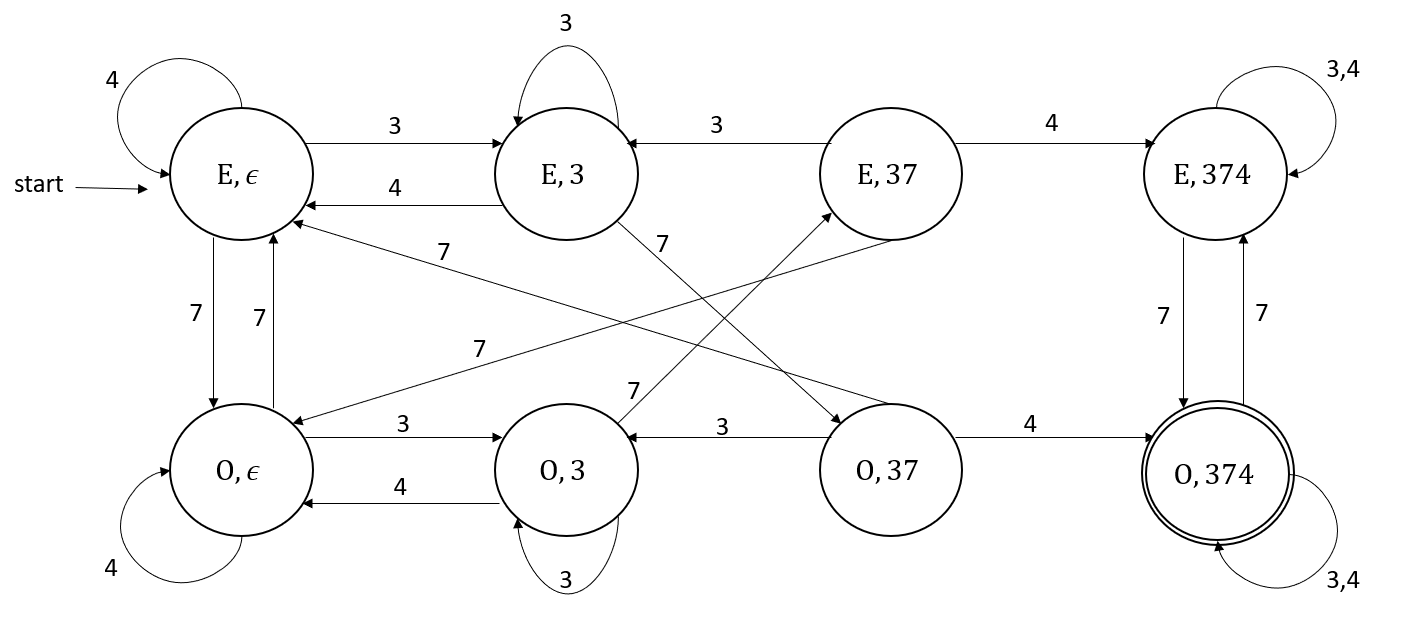
\includegraphics[width = 1\textwidth]{Q-7D}
\end{figure}

\question{7.E}

The folling NFA accepts the language. $q_0$ means maximal substring of consecutive $7$s is even and $q_1$ means maximal substring of consecutive $7$ is odd. When the substring of consecutive $7$s is odd and it reads $3$ or $4$. It will go to the rejecting state $\emptyset$. This makes sure that every maximal substring of consecutive $7$ is even in size.


\begin{figure}[hbt!]
	\centering
	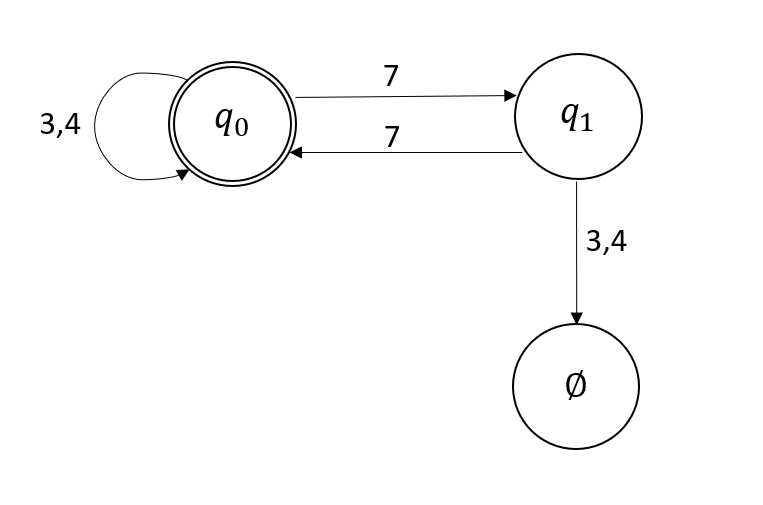
\includegraphics[width = 0.5\textwidth]{Q-7E}
\end{figure}

\question{8.A}\\
$\bullet$ \textbf{Intuition:} Just exchange all the "1" in the L with "$\epsilon$".\\
$\bullet$ \textbf{Answer:}Set NFA $N_1=(\sum_1,Q_1,\delta_1,s_1,A_1)$, then $N_1$ accepts DelOnes(L).
	
	$\bullet$ $Q_1 = Q$

	$\bullet$ $\delta_1(q,0) = \delta(q,0)$, $\delta_1(q,\epsilon) = \delta(q,1)$, $\delta_1(q,1) = \emptyset $

	$\bullet$ $s_1 = s$

	$\bullet$ $A_1 = A$\\
	

\question{8.B}\\
$\bullet$ \textbf{Intuition:} Construct two intermediate DFAs where $M_1$ represents $\{x\ \vline\ x \in L \}$ and $M_2$ represents $\{y\ \vline\ y^R \in L\}.$ $ThereAndBack(L)$ can be Constructed by concatenating these two languages.  For $M_2$, swap all the transition functions, the start state and the accepting states. Then connect the accepting states of $M_1$ with the new start state of $M_2$ by using $\epsilon$.\\
$\bullet$ \textbf{Answer:} Construct our NFA with "$\epsilon$" transitions between two DFAs. Then change the original q state to $(q,positive)$ or $(q,negative)$. positive means it's M in postive direction, negative means it's another M in reverse direction. 
	
	\begin{figure}[H]
	\centering 
	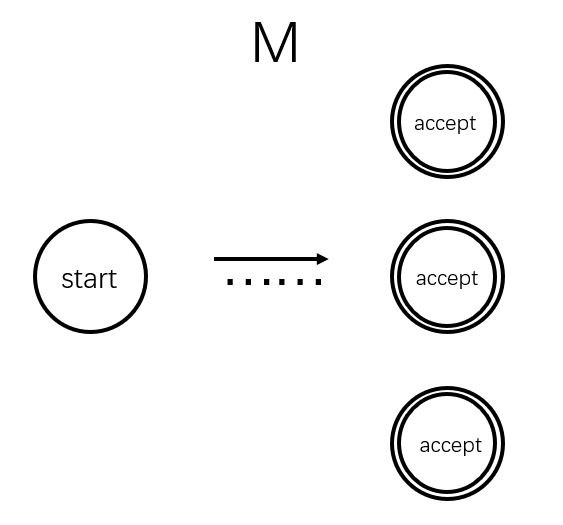
\includegraphics[height=5.5cm,width=6.5cm]{img//Q8B-1.png}
	\caption{M concept example figure}
   	\end{figure}
	\begin{figure}[H]
	\centering 
	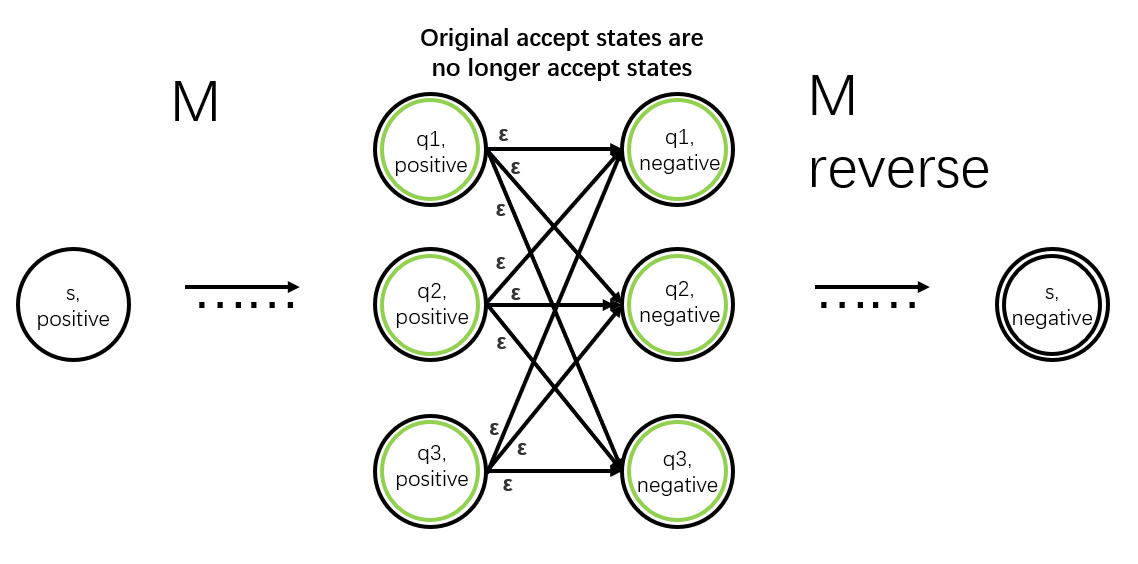
\includegraphics[height=5.5cm,width=12.5cm]{img//Q8B-2.png}
	\caption{N concept example figure}
   	\end{figure}

	These two figures just show the general ideas. The number of accepting states can be any. Set NFA $N_1=(\sum,Q_1,\delta_1,s_1,A_1)$,which accepts the language $ThereAndBack(L)$.
	
	$\bullet$ $Q_1 = 2Q \times \{positive,negative\}$

	$\bullet$  $\delta_1((q,positive),a) = (\delta(q,a),positive)$
 
	$\bullet$	$\delta_1( (\delta(q,a),negative),a) = (q,negative)$

	$\bullet$	$\delta_1((a_{pos},positive)$,$\epsilon) = \{(a_{neg},negative) \ \vline\ a_{neg} \in A\}$, \mbox{where }$a_{pos} \in A$

	$\bullet$ $s_1 = (s,postive)$

	$\bullet$ $A_1 = (s,negative)$\\

\question{8.C}\\
$\bullet$ \textbf{Intuition:} set the state to double state (q,r) so that it considers both x and y.\\
$\bullet$ \textbf{Answer:}Set $L_1=$XOR$(L)$, which is accepted by $N_1$.
Set $N_1=(\sum,Q_1,\delta_1,s_1,A_1)$\\

	$\bullet$ $Q_1 = Q \times Q$

	$\bullet$  $\delta_1((q,r),1) = \{(\delta(q,0),\delta(r,1)),(\delta(q,1),\delta(r,0))\}$, $\delta_1((q,r),0) = \{(\delta(q,1),\delta(r,1)),(\delta(q,0),\delta(r,0))\}$

	$\bullet$ $s_1 = (s,s)$

	$\bullet$ $A_1 = \{(q_1,q_2) \ \vline\ q_1 \in A$ and $q_2 \in A\}$\\



\question{9.A}

\noindent
Let $F$ be the language $(01)^\ast$. \\
Let $x$ and $y$ be arbitrary strings in $F$. \\
Then $x=(01)^i$ and $y=(01)^j$ for some non-negative integers $i\neq j$. \\ 
Let $z=(10)^i (01)^i$. \\
Then $xz=(01)^i(10)^i(01)^i \in L$. \\ 
And $yz=(01)^j(10)^i(01)^i \notin L$, because $i \neq j$. \\ 
Thus, $F$ is a fooling set for $L$. \\
Because $F$ is infinite, $L$ cannot be regular. \\

\question{9.B}

\noindent
Let $F$ be the language $\{0^{2n}10^n\ \vline\ n \ge 0\}$. \\
Let $x$ and $y$ be arbitrary strings in $F$. \\
Then $x=0^{2i}10^i$ and $y=0^{2j}10^j$ for some non-negative integers $i\neq j$. Assume $j > i$. \\
Let $z=0^i$. \\
Then $xz=0^{2i}10^{2i} \in L$. \\ 
And $yz = 0^{2j}10^{i+j}\notin L$, because $k(i + j) \neq 2j$ for any integar $k$.  \\
Thus, $F$ is a fooling set for $L$. \\
Because $F$ is infinite, $L$ cannot be regular. \\

\question{9.C}

\noindent
Let $F$ be the language $\{a^{2^n}\ \vline\ n \ge 0\}$. \\
Let $x$ and $y$ be arbitrary strings in $F$. \\
As $j=\log_{2}{i}$, $i=2^j$. \\
Then $x=a^{2^i}$ and $y=a^{2^j}$ for some non-negative integers $i\neq j$. \\
Let $z=b^i$. \\
Then $xz=a^{2^{i}}b^i \in L$. \\
And $yz=a^{2^j}b^i\notin L$, because $\log_{2}{2^j} \neq i$. \\
Thus, $F$ is a fooling set for $L$. \\
Because $F$ is infinite, $L$ cannot be regular. \\

\question{9.D}

\noindent
Let $F$ be the language $\{0^{3n^2}\ \vline\ n \ge 0\}$. \\
Let $x$ and $y$ be arbitrary strings in $F$. \\
Then $x=0^{3i^2}$ and $y=0^{3j^2}$ for some non-negative integers $i\neq j$. \\
Let $z=0^{i^2}0^{2i}$. \\ 
Then $xz=0^{4i^2}0^{2i} \in L$. \\
And $yz=0^{3j^2+i^2}0^{2i} \notin L$, because $i \neq j \Rightarrow \sqrt{3j^2 + i^2} \neq 2i$. \\
Thus, $F$ is a fooling set for $L$. \\
Because $F$ is infinite, $L$ cannot be regular. \\

\question{9.E}

\noindent
Let $F$ be the language $a^*c$. \\
Let $x$ and $y$ be arbitrary strings in $F$. \\
Then $x=a^ic$ and $y=a^jc$ for some non-negative integers $i\neq j$. \\
Let $z=d^i$. \\
Then $xz=a^icd^i \in L$. \\
And $yz=a^i cd^j \notin L$, because $i = \#_a(w) \neq j$, where $w$ is $a^i$. \\
Thus, $F$ is a fooling set for $L$. \\
Because $F$ is infinite, $L$ cannot be regular. \\

\end{document}
